\documentclass[crop,tikz]{standalone}% 'crop' is the default for v1.0, before it was 'preview'


% Tikz
\usepackage{tikz}
\usepackage{tkz-graph}
\usepackage{tikz-uml}
\usepackage{tikz-3dplot}
\usetikzlibrary{arrows,automata,calc,positioning,shadows.blur,decorations.pathreplacing,decorations.markings,pgfplots.groupplots}

\tikzstyle{class}=[
    rectangle,
    draw=black,
    text centered,
    anchor=north,
    text=black,
    text width=3cm,
    bottom color=white,
    top color=white]

% Cube drawing macros taken from here:
% https://tex.stackexchange.com/questions/489712/stacking-3d-cubes-with-spacing
\tikzset{plane/.style n args={3}{insert path={%
#1 -- ++ #2 -- ++ #3 -- ++ ($-1*#2$) -- cycle}},
unit xy plane/.style={plane={#1}{(1,0,0)}{(0,1,0)}},
unit xz plane/.style={plane={#1}{(1,0,0)}{(0,0,1)}},
unit yz plane/.style={plane={#1}{(0,1,0)}{(0,0,1)}},
get projections/.style={insert path={%
let \p1=(1,0,0),\p2=(0,1,0)  in
[/utils/exec={\pgfmathtruncatemacro{\xproj}{sign(\x1)}\xdef\xproj{\xproj}
\pgfmathtruncatemacro{\yproj}{sign(\x2)}\xdef\yproj{\yproj}
\pgfmathtruncatemacro{\zproj}{sign(cos(\tdplotmaintheta))}\xdef\zproj{\zproj}}]}},
pics/unit cube/.style={code={
\path[get projections];
\draw (0,0,0) -- (1,1,1);
\ifnum\zproj=-1
 \path[3d cube/every face,3d cube/xy face,unit xy plane={(0,0,0)}];
\fi
\ifnum\yproj=1
 \path[3d cube/every face,3d cube/yz face,unit yz plane={(1,0,0)}];
\else
 \path[3d cube/every face,3d cube/yz face,unit yz plane={(0,0,0)}];
\fi
\ifnum\xproj=1
 \path[3d cube/every face,3d cube/xz face,unit xz plane={(0,0,0)}];
\else
 \path[3d cube/every face,3d cube/xz face,unit xz plane={(0,1,0)}];
\fi
\ifnum\zproj>-1
 \path[3d cube/every face,3d cube/xy face,unit xy plane={(0,0,1)}];
\fi
}},
3d cube/.cd,
xy face/.style={fill=blue!10,fill opacity=1.},
xz face/.style={fill=blue!20,fill opacity=1.},
yz face/.style={fill=blue!30,fill opacity=1.},
num cubes x/.estore in=\NumCubesX,
num cubes y/.estore in=\NumCubesY,
num cubes z/.estore in=\NumCubesZ,
num cubes x=1,num cubes y/.initial=1,num cubes z/.initial=1,
cube scale/.initial=0.9,
every face/.style={draw},
/tikz/pics/.cd,
cube array/.style={code={%
 \tikzset{3d cube/.cd,#1}
 %\typeout{\NumCubesX,\NumCubesY,\NumCubesZ}
  \path[get projections];
  \ifnum\yproj=1
   \def\LstX{1,...,\NumCubesX}
  \else
   \ifnum\NumCubesX>1
    \pgfmathtruncatemacro{\NextToLast}{\NumCubesX-1}
    \def\LstX{\NumCubesX,\NextToLast,...,1}
   \else
    \def\LstX{1}
   \fi
  \fi
  \ifnum\xproj=-1
   \def\LstY{1,...,\NumCubesY}
  \else
   \ifnum\NumCubesY>1
    \pgfmathtruncatemacro{\NextToLast}{\NumCubesX-1}
    \def\LstY{\NumCubesY,\NextToLast,...,1}
   \else
    \def\LstY{1}
   \fi
  \fi
  \ifnum\zproj=1
   \def\LstZ{1,...,\NumCubesZ}
  \else
   \ifnum\NumCubesZ>1
    \pgfmathtruncatemacro{\NextToLast}{\NumCubesX-1}
    \def\LstZ{\NumCubesZ,\NextToLast,...,1}
   \else
    \def\LstZ{1}
   \fi
   \def\LstZ{\NumCubesZ,\NextToLast,...,1}
  \fi
  \foreach \X in \LstX
  {\foreach \Y in \LstY
   {\foreach \Z in \LstZ
    {\path (\X-\NumCubesX/2-1,\Y-\NumCubesY/2-1,\Z-\NumCubesY/2-1)
      pic[scale=\pgfkeysvalueof{/tikz/3d cube/cube scale}]{unit cube};}}
  }
}
}
}


\begin{document}

\tdplotsetmaincoords{85}{190} % the first argument cannot be larger than 90


\begin{tikzpicture}[
  auto,
  transform shape,
  block/.style={draw, align=center, minimum width=5em, minimum height=3.1em},
  annotation/.style={align=center, font=\tiny},
  line join=round,font=\sffamily,3d cube/.cd, num cubes x=1,num cubes y=1,num cubes z=1
  ]


\node (env) at (0, 0) {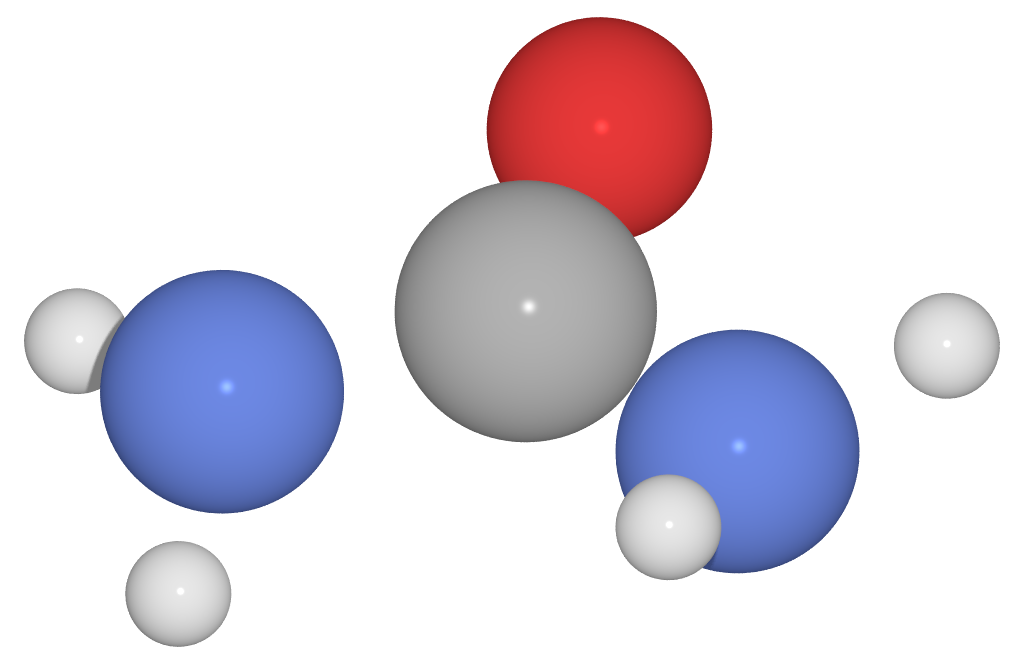
\includegraphics[width=2cm]{urea_3d.png}};
\begin{scope}[xshift=4cm,scale=1]
 \node[minimum width=2.2cm, minimum height=1.36cm] (features) {};
 \fill[draw=white,outer color=white,inner color=black!60!black,minimum width=3cm] (0.05,0.04) circle (0.15cm);
 \fill[draw=white,outer color=white,inner color=black!60!black,minimum width=3cm] (0.46,-0.24) circle (0.15cm);
 \fill[draw=white,outer color=white,inner color=black!60!black,minimum width=3cm] (0.32,-0.38) circle (0.15cm);
 \fill[draw=white,outer color=white,inner color=black!60!black,minimum width=3cm] (0.88,-0.04) circle (0.15cm);
 \fill[draw=white,outer color=white,inner color=black!60!black,minimum width=3cm] (-0.86,-0.04) circle (0.15cm);
 \fill[draw=white,outer color=white,inner color=black!60!black,minimum width=3cm] (-0.65,-0.51) circle (0.15cm);
 \fill[draw=white,outer color=white,inner color=black!60!black,minimum width=3cm] (-0.56,-0.12) circle (0.15cm);
 \fill[draw=white,outer color=white,inner color=black!60!black,minimum width=3cm] (0.18,0.4) circle (0.15cm);
\end{scope}

\begin{scope}[xshift=8cm, scale=0.42, tdplot_main_coords,local bounding box=moments]
  \path pic{cube array={num cubes x=4,num cubes y=4,num cubes z=4}};
\end{scope}
\begin{scope}[xshift=12cm, scale=0.42, tdplot_main_coords,local bounding box=invariants]
  \path pic{cube array={num cubes x=5}};
\end{scope}


% Links
\draw[<->,thick] ($(env.east) + (0.12, 0)$) -> ($(features.west) + (-0.12, 0)$);

\draw[<-,thick] ($(moments.west) + (-0.12, 0.1)$) -> ++(-1.6,0);

\draw[<->,thick] ($(moments.east) + (0.24, 0.1)$) -> ++(1.6,0);


% Inverse links
\draw[->,thick,draw=gray] ($(moments.west) + (-0.24, -0.1)$) -- ++(-1.6, 0);
% \draw[->,thick] ($(invariants.west) + (-0.2em, -0.3em)$) -- ($(moments.east) + (0.2em, -0.3em)$);
\draw[<-,thick,draw=gray] ($(moments.east) + (0.12, -0.1)$) -- ++(1.6, 0);


\begin{scope}[yshift=-1.4cm]
 \node (envs_label) {Environments};
 \node[anchor=north] at (envs_label.south) {$\{\vec{r}_i, Z_i, \ldots \}$};
 \node (features_label) at (4, 0) {Features};
 \node[anchor=north] at (features_label.south) {$f(\vec{r}_i, Z_i, \ldots)$};
 \node (moments_label) at (8, 0) {Moments};
 \node[anchor=north] at (moments_label.south) {$c_{nl}^m, m_{pqr}, \Omega_{nl}^m$};
 \node (invariants_label) at (12, 0) {Invariants};
 \node[anchor=north] at (invariants_label.south) {$\Phi_i$};
\end{scope}


%\draw[->,thick] (3.5, -3) -- ++(1,0) node[anchor=west] {$=$ analytical expression};
%\draw[->,thick,draw=gray] (3.5, -3.5) -- ++(1,0) node[anchor=west] {$=$ solved numerically};

\end{tikzpicture}

\end{document}
